\documentclass[11pt]{article}
\usepackage{amsmath, amssymb, amsthm}
\usepackage[retainorgcmds]{IEEEtrantools}

\usepackage[pdftex]{graphicx}
\usepackage{tikz}
\usepackage{circuitikz}
\usetikzlibrary{intersections,decorations.pathmorphing}

\usepackage{fancyhdr}

%Listings stuff
\usepackage{listings}
\usepackage{lstautogobble}
\usepackage{color}

\definecolor{gray}{rgb}{0.5,0.5,0.5}
\lstset{
basicstyle={\small\ttfamily},
tabsize=3,
numbers=left,
numbersep=5pt,
numberstyle=\tiny\color{gray},
stepnumber=2,
breaklines=true,
boxpos=t
}

%Format stuff
\pagestyle{fancy}
\headheight 35pt

%Header info
\chead{\Large \textbf{Coupled Oscillators}}
\lhead{}
\rhead{}

\begin{document}
\section{Equal-Mass 2-Oscillator System}
Consider a simple example with two identical SHO's connected by a spring.

\begin{center}
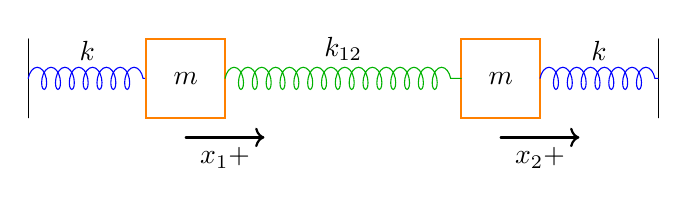
\begin{tikzpicture}
	[scale=1,line cap=round,
	%Styles
	axes/.style=,
	important line/.style={very thick},
	information text/.style={rounded corners,fill=red!10,inner sep=1ex},
	dot/.style={circle,inner sep=1pt,fill,label={#1},name=#1},
	spring/.style={decorate,decoration={coil,amplitude=4pt, segment length=5pt}}			
	]
	
	%Colors
	\colorlet{anglecolor}{green!50!black}	%angle arcs/lines
	
	%The graphic
	\draw (0,0) -- (0,1);
	\draw (8,0) -- (8,1);
	
	\draw[spring,blue] (0,.5) -- node[black,above=3pt]{$k$} (1.5,.5);
	\draw[orange,thick] (1.5,1) rectangle (2.5, 0);
	
	\draw[orange,thick] (5.5,1) rectangle (6.5, 0);
	\draw[spring,blue] (6.5,.5) -- node[black,above=3pt]{$k$} (8,.5);
	
	\draw[spring,green!70!black] (2.5,.5) -- node[black,above=3pt]{$k_{12}$} (5.5,.5);
	
	\node (m1) at (2, .5) {$m$};
	\node (m2) at (6, .5) {$m$};
	
	\draw[->,thick,black] (2,-.25) -- node[below]{$x_1 +$}(3, -.25);
	\draw[->,thick,black] (6, -.25) -- node[below]{$x_2 +$}(7, -.25);
\end{tikzpicture}
\end{center}

Free-body diagram analysis yields two coupled force equations.
\begin{IEEEeqnarray}{rCl}
	F_1 & = & -kx_1 - k_{12}(x_1 - x_2)\\
	F_2 & = & -kx_2 + k_{12}(x_1 - x_2)
\end{IEEEeqnarray}
Which leads to a system of two coupled homogeneous ODE's.
\begin{IEEEeqnarray}{rCl}
	m\ddot{x}_1 + (k + k_{12})x_1 - k_{12}x_2 & = & 0\\
	m\ddot{x}_2 + (k + k_{12})x_2 - k_{12}x_1 & = & 0
\end{IEEEeqnarray}

%\begin{center}
%\begin{tikzpicture}
%	[scale=3,line cap=round,
%	%Styles
%	axes/.style=,
%	important line/.style={very thick},
%	information text/.style={rounded corners,fill=red!10,inner sep=1ex},
%	dot/.style={circle,inner sep=1pt,fill,label={#1},name=#1}			
%	]
%	
%	%Colors
%	\colorlet{anglecolor}{green!50!black}	%angle arcs/lines
%	
%	%The graphic
%\end{tikzpicture}
%\end{center}

%	\begin{figure}[htb]
%		\centering
%		\includegraphics[width=0.8\textwidth]{filename.eps}
%		\caption{Caption.}
%		\label{fig:figure}
%	\end{figure}

%		\def\enotesize{\normalsize}
%		\theendnotes
\end{document}